\documentclass[letterpaper, 12pt]{article}
\usepackage[top=2cm,bottom=1cm,left=0.75in,right=0.75in,headheight=17pt, % as per the warning by fancyhdr
includehead,includefoot,
heightrounded, % to avoid spurious underfull messages
]{geometry}
\addtolength{\topmargin}{-.25in}
\usepackage{fancyhdr}
\pagestyle{fancy}
\usepackage{graphicx}
\usepackage{lastpage}
\usepackage{gensymb}
\usepackage{pgfplots}
\usepackage{MnSymbol,wasysym}


\begin{document}
\fancyhead[l]{	\includegraphics[height=1.2cm]{../Logo/sp.png} Name:}
\fancyhead[r]{REFERENCE MATERIAL}
\cfoot{\thepage\ of \pageref{LastPage}}
	


\begin{center}Things to Memorize: Graphing Motion
\end{center}
\subsection*{Basics of Graphs}
\begin{center}
	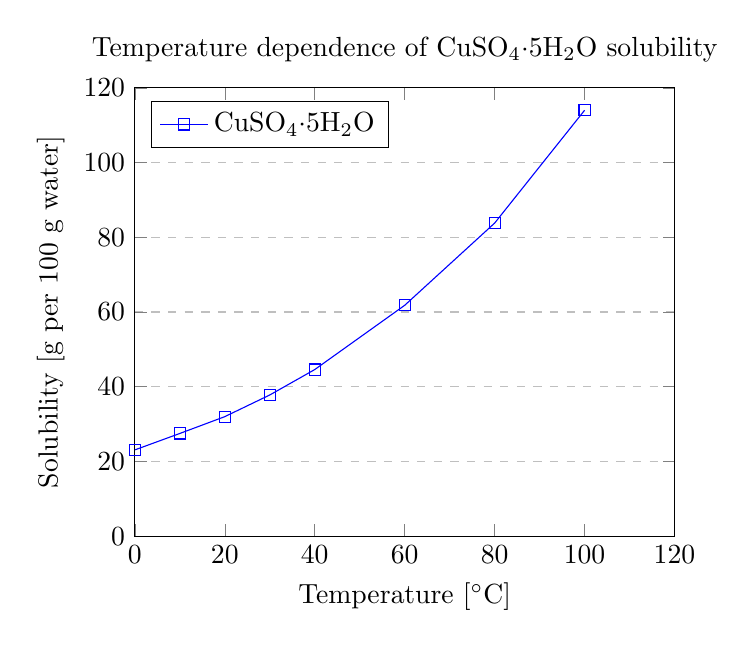
\begin{tikzpicture}
\begin{axis}[
title={Temperature dependence of CuSO$_4\cdot$5H$_2$O solubility},
xlabel={Temperature [$\degree$C]},
ylabel={Solubility [g per 100 g water]},
xmin=0, xmax=120,
ymin=0, ymax=120,
xtick={0,20,40,60,80,100,120},
ytick={0,20,40,60,80,100,120},
legend pos=north west,
ymajorgrids=true,
grid style=dashed,
]

\addplot[
color=blue,
mark=square,
]
coordinates {
	(0,23.1)(10,27.5)(20,32)(30,37.8)(40,44.6)(60,61.8)(80,83.8)(100,114)
};
\legend{CuSO$_4\cdot$5H$_2$O}

\end{axis}
\end{tikzpicture}
\end{center}

\begin{itemize}
	\item Graphs should include the following things:
		\begin{itemize}
			\item A Title that describes what the graph is about.
			\item Labels and units on each axis.
			\item Numbers should be evenly spaced at regular intervals.
			\item All data should be within the graph, and should take up at least half of the graph.
		\end{itemize}
	\item Don't connect the dots of data from an experiment.  Instead, draw a \textbf{Best-Fit Line} or \textbf{Best-Fit Curve} through your data points. 

	\item To find the slope of a graph, use the slope formula: $m = \frac{y_2 - y_1}{x_2-x_1}$
	\item To find area under the line or curve:
		\begin{itemize}
			\item approximate it using
		
	 		\begin{itemize} 
	 			\item rectangles ($A = b \times h  $)
	 			\item triangles ($A = \frac{1}{2} b \times h $)
	 			\item trapezoids ($A = (\frac{b_1+b_2}{2}) \times h $)  
	 		\end{itemize}
	 		\item If you know the equation and some calculus, you can find $\int_{A}^{B} f(x) dx $
	 	\end{itemize}
	 		

\end{itemize}
\vspace{1in}

\subsection*{Position vs Time Graphs}
\begin{itemize}
	\item To determine how far from the detector an object is located, look at the vertical axis of the position-time graph.
	\item To determine how fast an object is moving, look at the slope of the position-time graph.
	\item To determine which way the object is moving, look at which way the position-time graph is sloped.
	\begin{itemize} 
		\item A position-time graph with a positive slope (like a forward slash /) means the object is moving in the positive direction (away from the detector).
		\item A position-time graph with a negative slope (like a back slash $\backslash$)  means the object is moving in the negative direction (toward the detector).
		\end{itemize} 
	\item To determine the type of acceleration an object is moving with, look at how the graph is curved.
	\begin{itemize}
		\item A straight line on a position-time graph means that the object is not accelerating.
		\item A curve that is concave-up (like the mouth of a \smiley) on a position-time graph means the object has positive acceleration.
		\item A curve that is concave-down (like the mouth of a \frownie) on a position time graph means the object has negative acceleration. 
	\end{itemize}
\end{itemize}

\subsection*{Velocity vs Time Graphs}
\begin{itemize}
	\item To determine how fast an object is moving, look at the vertical axis of the velocity-time graph.
	\item To determine which way the object is moving, look at whether the velocity-time graph is above or below the horizontal axis.
	\begin{itemize}
		\item  An object is moving in the positive direction (away from the detector) if the velocity-time graph is above the horizontal axis.
		\item An object is moving in the negative direction (toward the detector) if the velocity-time graph is below the horizontal axis.  
		\end{itemize}
	\item To determine how far an object travels, determine the area between the velocity-time graph and the horizontal axis.
	\item On a velocity-time graph it is not possible to determine how far from the detector the object is located.
	\item Most everyday motion can be represented with straight segments on a velocity-time graph.
	
	
\end{itemize}

	


\end{document}
